\documentclass[12pt]{article} % Default font size is 12pt, it can be changed here

\usepackage[utf8]{inputenc} % utf8 encoding
\usepackage{geometry} % Required to change the page size to A4
\geometry{a4paper} % Set the page size to be A4 as opposed to the default US Letter

\usepackage{graphicx} % Required for including pictures

\usepackage{float} % Allows putting an [H] in \begin{figure} to specify the exact location of the figure

\linespread{1.2} % Line spacing

%\setlength\parindent{0pt} % Uncomment to remove all indentation from paragraphs

\graphicspath{{pictures/}} % Specifies the directory where pictures are stored

\usepackage{listings} % To be able to have code in text
\usepackage{color} % To be able to have colors

\definecolor{codegreen}{rgb}{0,0.6,0}
\definecolor{codegray}{rgb}{0.5,0.5,0.5}
\definecolor{codepurple}{rgb}{0.58,0,0.82}
\definecolor{backcolour}{rgb}{0.95,0.95,0.92}
 
\lstdefinestyle{codestyle}{
    backgroundcolor=\color{backcolour},   
    commentstyle=\color{codegreen},
    keywordstyle=\color{magenta},
    numberstyle=\tiny\color{codegray},
    stringstyle=\color{codepurple},
    basicstyle=\footnotesize,
    breakatwhitespace=false,         
    breaklines=true,                 
    captionpos=b,                    
    keepspaces=true,                 
    numbers=left,                    
    numbersep=5pt,                  
    showspaces=false,                
    showstringspaces=false,
    showtabs=false,                  
    tabsize=2
}
 
\lstset{style=codestyle}

\begin{document}

%----------------------------------------------------------------------------------------
%   TITLE PAGE
%----------------------------------------------------------------------------------------

\begin{titlepage}

\newcommand{\HRule}{\rule{\linewidth}{0.5mm}} % Defines a new command for the horizontal lines, change thickness here

\center % Center everything on the page

\textsc{\LARGE Lund University, Faculty of Engineering}\\[1.5cm] % Name of your university/college
\textsc{\Large EDAF05}\\[0.5cm] % Major heading such as course name
\textsc{\large Algorithms, data structures, and complexity}\\[0.5cm] % Minor heading such as course title
{\large \today}\\[3cm] % Date, change the \today to a set date if you want to be precise

\HRule \\[1cm]
{ \huge \bfseries Summary of EDAF05}\\[0.4cm] % Title of your document
\HRule \\[1.5cm]

\emph{Author:} Fred \textsc{Nordell} % Your name

{\large \today}\\[3cm] % Date, change the \today to a set date if you want to be precise

%\includegraphics{Logo}\\[1cm] % Include a department/university logo - this will require the graphicx package

\vfill % Fill the rest of the page with whitespace

\end{titlepage}

%----------------------------------------------------------------------------------------
%   TABLE OF CONTENTS
%----------------------------------------------------------------------------------------

\tableofcontents % Include a table of contents
\lstlistoflistings % Include a table of lstlistings

\newpage % Begins the essay on a new page instead of on the same page as the table of contents 


\section{Algorithms} % Major section

This section will describe the diffrent problems and algorithms covered in the course.

\subsection{Stable Marriage} % Sub-section
Given two sets $X = {x_{1}, x_{2}, \dots x_{n}}$ and $Y = {y_{1}, y_{2}, \dots y_{n}}$ a mathcing $M$ is a set of pairs $(x_{i}, y_{j})$ such that an $x \in X$ and an $y \in Y$ appear in most one pair. Thus it follows that a matching does not let anybody have multiple partners.

\par If the size of $M$ is $n$ it is called a \textbf{perfect matching} (All members of $X$ and $Y$ were matched). Hovever a perfect match is insufficient. All $x$ and $y$ have a preferred list, sorted in descending order, of the opposite set. The matching $M$ is considered \textbf{unstable} if it contains to pairs where they would rather switch partners. \textit{i.e.}\\
$x_{i}$ prefers $y_{j}$ and $y_{j}$ prefers $x_{i}$ \\
or \\
$y_{p}$ prefers $x_{q}$ and $x_{q}$ prefers $x_{p}$ \\
Is it always possible to find a stable matching with no unstable pairs?

\subsubsection{The Gale-Shapely algorithm}
As each person has a preferred list of partners each $x$ just needs to remember the position in the list. But as $y$ has to accept $y$ has to check if $x$ is before the current matched $x_{y}$. This may need $O(n)$ operations. A naive implementation of this algorithm may have a time complexity of $O(n^3)$ as each $x$ tries to match with each $y$ and each ask take $O(n)$ time. To reduce time complexity each $y$ should not save a prefence list, instead they should save an inverted list. Thus \texttt{[3, 2, 4, 1]} means that $x_{1}$ comes at position 3 and $x_{4}$ comes at position 1. This reduces the operation to constant time. Below is a Java implementation of the Gale-Shapely algorithm.

\begin{lstlisting}[language=Java]
public String match() {
        for(Person p: persons) {
            if(p.getId() % 2 == 0) {
                y.add(p);
            } else {
                x.addLast(p);
            }
        }
        while(x.size() > 0) {
            Person m = x.removeFirst();
            int w = (m.getPrefered()/2)-1;
            if(y.get(w).matched == null) {
                y.get(w).matched = m;
                m.matched = y.get(w);
            } else if(y.get(w).compareMatched(m)) {
                x.addLast(y.get(w).matched);
                y.get(w).matched = m;
                m.matched = y.get(w);
            } else {
                x.addLast(m);
            }
        }
        StringBuilder sb = new StringBuilder();
        for (Person w : y) {
            sb.append(w.matched.name + " -- " + w.name + "\n");
        }
        return sb.toString();
    }
\end{lstlisting}

\subsection{Graphs} % Sub-section
\begin{figure}[H]
\center{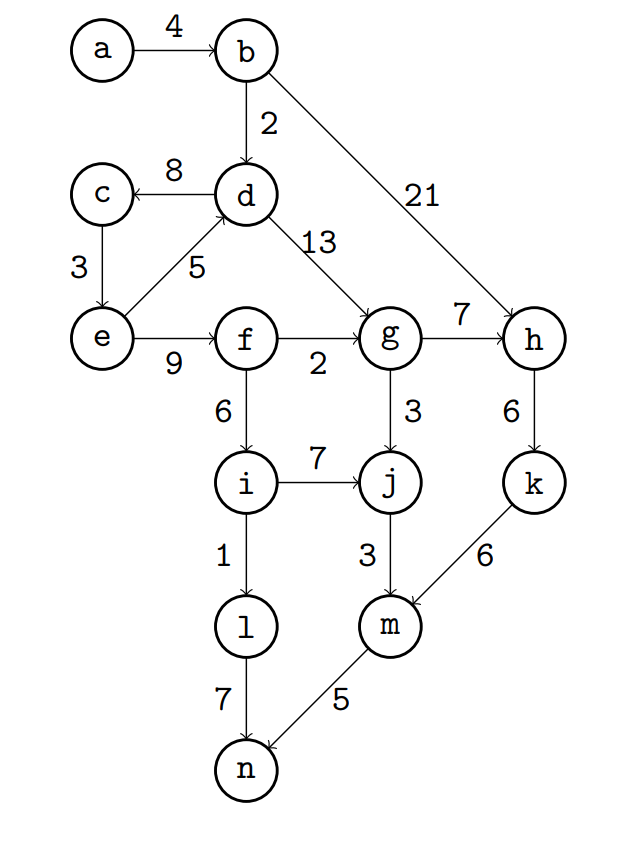
\includegraphics[width=0.5\linewidth]{graph}}
\caption{Example graph.}
\label{exGraph}
\end{figure}
A graph is a set of nodes $V$ and a set of edges $E$. Edges connects nodes toghether. A graph which edges you are able to follow from one to another but not backwards is called a \textbf{directed graph}. In contrary a graph whos edges connections both to and from a node is called an \textbf{undirected graph}. An undirected graph is \textbf{connected} if there is a path between every pair of nodes. A \textbf{cycle} is a path which terminates in the start node. In a connected graph there is no unreachable nodes. A graph is said to be disconnected if there exists two nodes in $G$ such that no path in $G$ has those two nodes as endpoints. A graph with one vertex is connected. An edgeless graph with two or more vertecies is disconnected.

\subsubsection{Bipartite graphs}
A bipartite graph is a graph taht can be colored with two colors such that every ege connects two nodes with different colors.

\begin{figure}[H]
\center{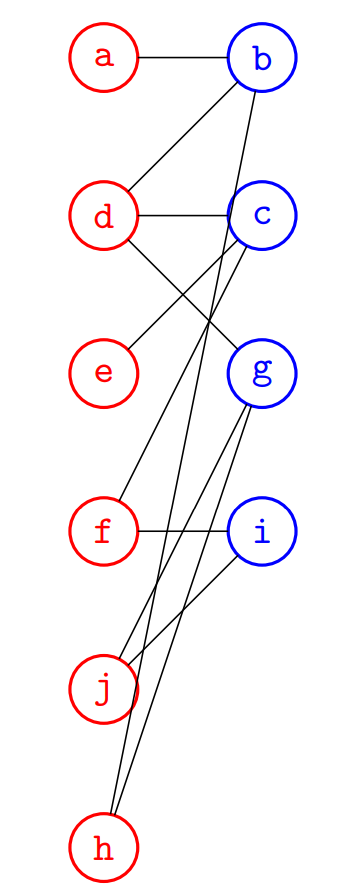
\includegraphics[width=0.5\linewidth]{bipartite}}
\caption{Example bipartite graph.}
\label{exBiGraph}
\end{figure}

\subsubsection{BFS and DFS}
The problem is to find a path from $s$ to $t$. There are two different approches, breath first and depth first. Depth first explores all possible branches first and the n backtracks to find the shortest path if there is any. Breath first is the opposite, you explore the closest nodes first and then explore one level deeper. Basically like rippels on a lake, start close and propagate outwards until you hit your target.

\par Time complexity of DFS is $O(V + E)$ and of BFS is $O(V + E)$, how neat.

\begin{lstlisting}[language=Python, caption=Recursive DFS in Python]
def DFS(G,v):
    label v as discovered
    for all edges from v to w in G.adjacentEdges(v) do
        if vertex w is not labeled as discovered then
            recursively call DFS(G,w)
\end{lstlisting}

\begin{lstlisting}[language=Python, caption=BFS in Python]
def BFS(G,v,target):
    create empty set Visited
    Q = new Stack()
        Q.append(v)                      
        while Q is not empty:
            current = Q.pop()
            if current.value == target:
                    return current
            for each node n that is adjacent to current:
                    if n is not in Visited:
                    Q.enqueue(n)
\end{lstlisting}

\subsection{Greedy algorithms} % Sub-section
The definition is not trivial. Main idea is to make the best local decision at a potential cost at the global level. Herein lies the problem of finding the rule which solves the problem optimally. There are two ways we can prove optimallity. 
\begin{enumerate}
\item If the greedy algorithm is at least as good as an optimal solution we know it is also optimal
\item Exchange argument -- transform the output of an optimal algorithm to the output of the greedy algorithm
\end{enumerate}

\subsubsection{Greedy graph algorithms}
How do we find the shortest path in a given graph? to every other node? Can we find this efficiently? Edges have weights which can be both negative and positive (although easier with positive).

\subsubsection{Dijkstra's algorithm}
Given a directed graph $G(V, E)$ a weight function $w: E -> R$ and a node $s \in V$ Dijkstra's algorithm computes the path to every other node. To find the path to a specific node traverese backwards until v. Alternitavly implement a condition where the algorithm ends when the target is found.
\par Assume $n$ nodes and $m$ edges, the running time is $O(m \cdot log(n))$. Below is a python/pseudocode implementation.

\begin{lstlisting}[language=Python, caption=Dijkstra's in pseudo/Python]
node n = (value, edges)
def Djigstra(G,n,target):
    n.value = 0; #sets the start nodes value to 0, All other nodes should have inf as value. 
    Visited = {}
    while n != target:
        for Eedges connected to n not in Visited:
            if n.value + edge.value < edge.end.value:
                edge.end.value= n.value + edge.value
        Visited.append(n)
        n = nextNode #pickout a node not in visited connected to n
    return n.value
\end{lstlisting}

\subsubsection{Prim's algorithm}
Assume the nodes are cities and a country wants to connect the cities to a electrical network. We want to find a subset of edges where all cities are connected at minimal cost i.e. we want to find the \textbf{minimum-wheight spanning tree}.
\par Given a undirected graph $G(V,E)$ $T \subseteq E$ and $(V, T)$ is a tree it is called a \textbf{spanning tree} of $G(V, E)$. If the edge costs are minimized, it is a \textbf{MST}. Prim's algorithm is similar to Dijkstra's as it builds one $MST$. At the core there is the problem if it is safe to add an edge. A partition $(S, V - S)$ of the nodes $V$ is called a \textbf{cut}. An edge $(u, v)$ crosses the cut if $u \in S$ and $v \in V - S$, that $u$ and $v$ are in different parts of the partition. How to determine safeness is in lecture slides. The running time of Prim's is $O(m \cdot log(n))$

\begin{lstlisting}[language=Scala, caption=Prim's in scala]
class Node(id: String, var cost: Int = Int.MaxValue, var leastEdge: Edge = null) extends Ordered[Node]{
  var edges = scala.collection.mutable.PriorityQueue[Edge]()

  def compare(that: Node) = cost compare that.cost

  def addEdge(from: Node, to: Node, weight: Int): Unit = {
      edges.enqueue(new Edge(from, to, weight))
  }
  override def toString: String = id
}
class Edge(val from: Node, val to: Node, val weight: Int) extends Ordered[Edge]{

    def compare(that: Edge) = that.weight compare weight

    override def toString: String = from + "<-->" + to + " ("+ weight +")"

}
def prim(g: List[Node]): scala.collection.mutable.HashSet[Node] = {
    var mst_nodes = scala.collection.mutable.HashSet[Node]()
    val pq = new java.util.PriorityQueue[Node](g.asJava)
    pq.peek().cost = 0
    while(!pq.isEmpty) { //O(n)
      val node = pq.poll()
      mst_nodes += node
      node.edges.foreach(e => //snitt O(m/n)
        if (!(mst_nodes contains e.to)) {
          if (e.to.cost > e.weight) {
            e.to.cost = e.weight
            e.to.leastEdge = e
            pq.remove(e.to) //log(n)
            pq.offer(e.to)
          }
        }
      )
    }
    return mst_nodes //multiplicera sakerna => O(m*log(n))
  }
\end{lstlisting}

\subsubsection{Kruskal's algorithm}
Kruskal's algorithm builds a forest that later becomes one MST. The running time is $O(e \cdot log(v))$ where $v$ is the verticies and $e$ is the edges in the graph $G(V, E)$. 

\begin{lstlisting}[language=Python, caption=Kruskal in python]
def kruskal(V,E):
sort(E) //Sorts E, low to high
forest = {}
while E.length != 0:
    edge = E.pop()
    if edge has no endpoint in the forest:
        forest.append(edge)
return forest
\end{lstlisting}

\subsection{Divide and Conquer}
Divide and conquer is the technique of dividing a hard problem to multiple easier problems and then solving those. Suppose we have a problem which can be solved in $O(n^2)$ time, if we divide this problem into two subproblems in linear time and sove those problems and then combine the results in linear time the running time becomes $O(n \cdot log(n))$. Some examples include Mergesort, calculation of fibbonaci numbers or finding the largest perfect subtree in a binary search tree.

\begin{lstlisting}[language=Python, caption=Fibbonaci in Python]
#find the n:th number in the fibbonaci sequence.
def fibbonacis(number n):
    if n =< 1:
        return fibbonacis(n-1) + fibbonacis(n-2)
    else:
        return 1
\end{lstlisting}
\begin{lstlisting}[language=Python, caption=Perfect subtree in BST]
def func(node n):
    if(n!=None):
        tuple = (func(n.left),func(n.right))
        MyMax = 1+ min(tuple[0],tuple[1])
        TotalMax = max(MyMax,tulp[0],tuple[1])
        return (myMax,TotalMax);
    else:
        return (0,0)
\end{lstlisting}

\subsection{Dynamic programming} % Sub-section
Dynamic programming is closely related to divide and conquer but with some crucial differences. In divide and conquer we solve \textbf{indepentent} subproblems but in Dynamic programming we solve \textbf{overlapping} subproblems. The idea is to avoid computing already computed subproblems, but rather to store the already computed subproblems and acces that when the same problems comes up again. This technique of storing the solutions is called \textit{Memoization}.

\par Dynamic programming is often used to optimize problems as it uses the alrady computed subproblems and combines them to give the best solution for the problem. Which, in contrast to a Greedy algorithm which pciks the locally optimal choice at each step does not guarantee an optimal solution but is often fast to calculate.

\par The fibbonaci example can be improved upon as the memory cost of large n for a recursive solution is large. With dynamic programming we can reduce this to $O(n)$ time complexity and space, this is because we remember each solution in for example an array. The Array can then be used to calculate the next numbers.

\begin{lstlisting}[language=Python, caption=Dynamic programming Fibbonaci numbers in Python]
def fibbonaci(n):
    array ={}
    array[0] = 0
    array[1] = 1
    for i in range(2,n):
        array[i] = array[i-1] + array[i-2]

    return array
\end{lstlisting}

\subsection{Network flow} % Sub-sub-section
Network flow problems are similar to Graph problems, but in network flow problems every edge has a weight or rather a capacity. There exists a source node $s$ with no predecessor and a sink node $t$ with no sucessor.

\begin{figure}[H]
\center{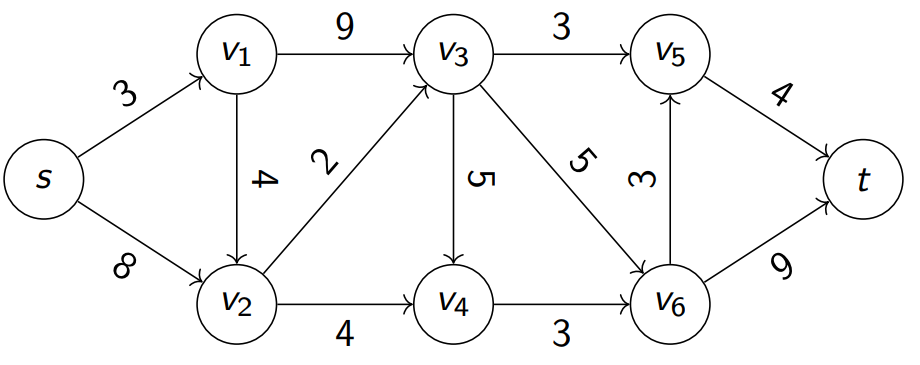
\includegraphics[width=0.5\linewidth]{flow}}
\caption{Example network flow graph.}
\label{flow}
\end{figure} 

\paragraph{Terminology}
\begin{itemize}
    \item \textbf{cut}: is a partion $(A, B)$ with $s \in A$ and $t \in B$
    \item \textbf{capacity} of a cut: $cap(A, B) = \sum_{e out from A} c(e)$
    \item \textbf{min-cut problem}: to find a cut of minimum capacity
    \item \textbf{flow} a function of how much of the capacity is used
    \item \textbf{capacity constraint} for each $e \in E, 0 \leq f(e) \leq c(e)$, an edge cannot have more flow than it's capacity
    \item \textbf{flow conservation constraint}: the flow coming in to a vertex $v$ must equal the flow going out from $v$, does not apply to source and sink.
    \item \textbf{maximum flow problem}: find a flow $f$ with maximum value
\end{itemize}

\par The \textbf{max-flow min-cut} theorem states that in the flow network you can calculate the maximum flow from $s$ to $t$ using the weight of the \textbf{minimum cuts}. That is, the weight of the edges that if removed would disconnect the source from the sink adds upp to the maximum flow from $s$ to $t$.

\subsubsection{Ford-Fulkeson algorithm}


\begin{thebibliography}{99} % Bibliography - this is intentionally simple in this template

\bibitem[Figueredo and Wolf, 2009]{Figueredo:2009dg}
Figueredo, A.~J. and Wolf, P. S.~A. (2009).
\newblock Assortative pairing and life history strategy - a cross-cultural
  study.
\newblock {\em Human Nature}, 20:317--330.
 
\end{thebibliography}

%----------------------------------------------------------------------------------------

\end{document}